\documentclass{article}
\usepackage[utf8]{inputenc}
\textheight = 25cm 
\textwidth = 15cm
\topmargin = -3.0cm 
\oddsidemargin = 1.5cm
\usepackage{hyperref}
\hypersetup{
    colorlinks=true,
    linkcolor=blue,
    filecolor=blue,
    citecolor=black,      
    urlcolor=blue,
    }

\usepackage{float}
\usepackage{graphicx}

\usepackage{amsmath}
\usepackage{amssymb}
\usepackage{amsfonts}
\usepackage{mathtools, xparse}
\usepackage[shortlabels]{enumitem}

\usepackage[many]{tcolorbox}
\usepackage{lipsum}

\title{Tarea 2 Matemáticas Avanzadas de la Física}
\author{Cerritos Lira Carlos}
\date{25 de Marzo del 2020}

\begin{document}
\maketitle
Nota: código utilizado se encuentra en 
\url{https://github.com/carloscerlira/MAF/blob/master/Tarea_2/code.ipynb}
\section*{1.-}
Usar la transformada de Laplace para resolver las siguientes ecuaciones diferenciales
con condiciones iniciales y estudiar la gráfica de las soluciones.
\begin{enumerate}[a)]
    \item $y'' + 3y' + 2y = -5sin(t) + 5cos(t),\quad y_0 = 5,\quad y'_0 = 3$
    \item $y'' + y = 5u(t-\pi),\quad y_0=2,\quad y'_0 = 4$, donde $u(t)$ es la función de Heaviside.
    \item $y'' + 2y' + 2y = e^{-t} + 5\delta (t-2),\quad y_0 = 0,\quad y'_0=1$, donde $\delta(t)$ es la delta de Dirac.
    \item $ y'' + 8y' + 15y = 
    \begin{cases*}
        35e^{2t}, & si $0<t<2$ \\
        0,& caso contrario
    \end{cases*},\quad y_0=3, \quad y'_0=-8 $

\end{enumerate}
\begin{tcolorbox}[breakable]
    \subsubsection*{Caso General}
    En el caso general se tiene:
    \begin{align*}
        Ay'' + By' + Cy &= f(t)\\
        A(p^2Y - py_0 - y_0') + B(pY - y_0) + CY &= F \\
        Y(Ap^2 + Bp + C) - (Ay_0p + Ay_0' + By_0) &= F \\
        Y &=\frac{1}{A(p+a)(p+b)}(F + Ay_0p + Ay_0' + By_0) \\
        Y &=\frac{1}{A}H(F + G) = \frac{1}{A} (Y_1 + Y_2) 
    \end{align*} 
    Resolvamos $Y_1 = HF$ \\ 
    En este caso tenemos $y_1 = f*h$, donde 
    \begin{align*}
        h(t) &=\frac{e^{-at} - e^{-bt}}{b-a},\quad a \neq b \\ 
        h(t) &=te^{-at},\quad a=b
    \end{align*}
    Resolvamos $Y_2 = HG$. \\
    En este caso tenemos $y_2 = h*g$, donde 
    \begin{align*}
        g &=Ay_0\delta' + (Ay_0' + By_0)\delta
    \end{align*}
    calculando la convolución obtenemos:
    \begin{align*}
        h*g &=Ay_0 \delta'*h + (Ay_0' + By_0) \delta*h \\
        h*g &=Ay_0h' + (Ay_0' + By_0)h
    \end{align*}
    entonces la solución es $y = \frac{1}{A} (y_1 + y_2)$
    \subsubsection*{a)}
    Hacemos cuentas para encontrar los parametros del caso general:
    \begin{align*}
        Ap^2 + Bp + C 
        &= p^2 + 3p + 2 \\
        &= (p+1)(p+2) 
    \end{align*}
    se tiene entonces:
    \begin{align*}
        &f(t) = -5sint + 5cost
        &&A, B, C = 1, 2, 3 \\ 
        &y_0, y_0' = 5, 3 
        &&a, b = 1, 2 
    \end{align*}
    entonces nuestra solución es:
    \begin{align*}
        y 
        &= h*f + h*g \\
        &= \int_{0}^t h(t-\tau)f(\tau)d\tau  + Ay_0h' + (Ay_0'+By_0)h 
    \end{align*}
    resolviendo numéricamente $h*f$ encontramos la gráfica de $y$:
    \begin{figure}[H]
        \centering
        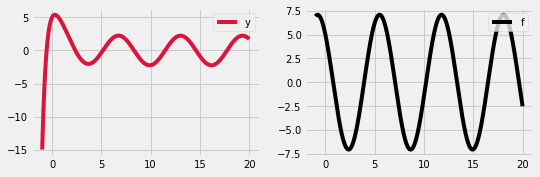
\includegraphics[scale=0.7]{images/p1_1.png}
    \end{figure}

    \subsubsection*{b)}
    Hacemos cuentas para encontrar los parametros del caso general:
    \begin{align*}
        Ay^2 + By + C 
        &= y^2 + y \\
        &= (y+1)(y+0)
    \end{align*}
    se tiene entonces:
    \begin{align*}
        &f(t) = 5u(t-\pi) 
        &&A, B, C = 1,1,0 \\
        &y_0, y_0' = 2, 4 
        &&a,b = 1,0 
    \end{align*}
    entonces nuestra solución es:
    \begin{align*}
        y 
        &= h*f + h*g \\
        &= \int_{0}^t h(t-\tau)f(\tau)d\tau  + Ay_0h' + (Ay_0'+By_0)h 
    \end{align*}
    resolviendo numéricamente $h*f$ encontramos la gráfica de $y$:
    \begin{figure}[H]
        \centering
        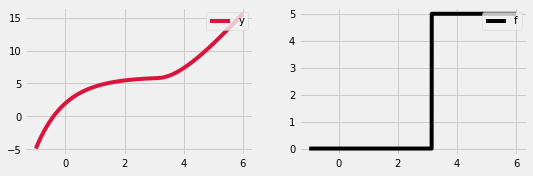
\includegraphics[scale=0.7]{images/p1_2.png}
    \end{figure}
    \subsubsection*{c)}
    Hacemos cuentas para encontrar los parametros del caso general:
    \begin{align*}
        Ay^2 + By + C 
        &= y^2 + 2y + 2 \\
        &= (y+1+i)(y+1-i)
    \end{align*}
    se tiene entonces:
    \begin{align*}
        &f(t) = e^{-t} + 5\delta(t-2)
        &&A, B, C = 1, 2, 2 \\ 
        &y_0, y_0' = 0,1
        &&a,b = 1+i, 1-i   
    \end{align*}    
    entonces nuestra solución es:
    \begin{align*}
        y
        &= h*f + h*g \\
        &= \int_{0}^t h(t-\tau)e^{-\tau}d\tau + 5h(t-2)u(t-2)  + Ay_0h' + (Ay_0'+By_0)h 
    \end{align*}
    resolviendo numéricamente $h*e^{-t}$ encontramos la gráfica de $y$:
    \begin{figure}[H]
        \centering
        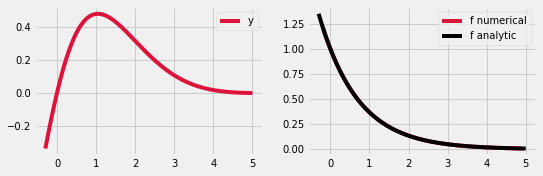
\includegraphics[scale=0.7]{images/p1_3.png}
    \end{figure}

    \subsubsection*{d)}
    Hacemos cuentas para encontrar los parametros del caso general:
    \begin{align*}
        Ay^2 + By + C 
        &= y^2 + 8y + 15 \\
        &= (y+5)(y+3)
    \end{align*}
    se tiene entonces:
    \begin{align*}
        &f(t) = 
        \begin{cases*}
            35e^{2t}, & si $0<t<2$ \\
            0,& caso contrario
        \end{cases*}
        &&A, B, C = 1,8,15 \\
        &y_0, y_0' = 3,-8
        &&a,b = 5,3 
    \end{align*}
    entonces nuestra solución es:
    \begin{align*}
        y(t) 
        &= h*f + h*g \\
        &= \int_{0}^t h(t-\tau)f(\tau)d\tau + Ay_0h' + (Ay_0'+By_0)h 
    \end{align*}
    resolviendo numéricamente $h*f$ encontramos la gráfica de $y$:
    \begin{figure}[H]
        \centering
        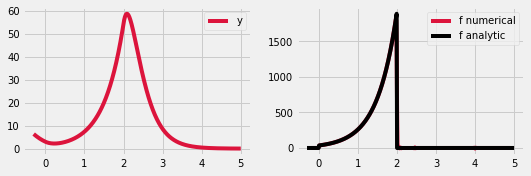
\includegraphics[scale=0.7]{images/p1_4.png}
    \end{figure}
\end{tcolorbox}
\newpage

\section*{2.-}
Se define el siguiente conjunto de funciones (llamado lorentziano):
\[
f_\epsilon(t)=\frac{1}{\pi}\frac{\epsilon}{t^2+\epsilon^2}, t\in\mathbb{R}, 
\epsilon \ge>0.
\]
\begin{enumerate}[a)]
    \item Argumentar que $\lim_{\epsilon \to 0^+}f_\epsilon(t)=\delta(t)$, 
    donde $\delta(t)$ es la delta de Dirac. 
    \item A partir de $f_\epsilon(t)$ obtener un conjunto de funciones que aproximen a la función de Heaviside $h(t)$, a $\delta'(t)$ y 
    a $\delta''(t)$ y estudiar las correspondientes gráficas. 
\end{enumerate}
\begin{tcolorbox}[breakable]
    \subsubsection*{a)}
    Nuestro conjunto de funciones debe de satisfacer:
    \begin{align*}
        \lim_{\epsilon \to 0^+} \int_{-\infty}^\infty f_\epsilon g dt &= g(0)
        \quad \forall g \in S(R)
    \end{align*}
    esto sucede si se cumplen las relaciones: 
    \begin{align*}
        \int_{-\infty}^\infty f_{\epsilon}dt &= 1, \quad \forall \epsilon > 0 \\
        \lim_{\epsilon \rightarrow 0^+}f_\epsilon (t) &= 0, \quad \forall t \neq 0 \\
        \lim_{\epsilon \rightarrow 0^+}f_\epsilon (0) &= \infty
    \end{align*}
    para la primera relación:
    \begin{align*}
        \int_{-\infty}^\infty f_{\epsilon}dt 
        &= \frac{1}{\pi} arctan\frac{t}{\epsilon} \biggr\rvert_{-\infty}^\infty \\
        &= \frac{1}{\pi} \pi = 1
    \end{align*}
    para la segunda relación:
    \begin{align*}
        \lim_{\epsilon \rightarrow 0^+} f_\epsilon (t) 
        &=\frac{1}{\pi} \lim_{\epsilon \rightarrow 0^+} \frac{\epsilon}{t^2} \\ 
        &= 0
    \end{align*}
    para la tercer relación:
    \begin{align*}
        \lim_{\epsilon \rightarrow 0^+} f_\epsilon (t) 
        &=\lim_{\epsilon \rightarrow 0^+} \frac{1}{\pi} \frac{1}{\epsilon} \\
        &= \infty
    \end{align*}
    \begin{figure}[H]
        \centering 
        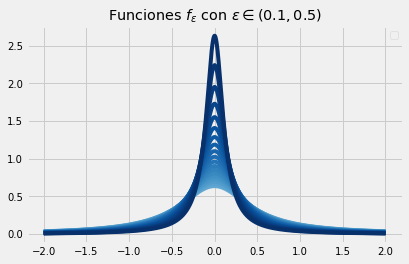
\includegraphics[scale=0.7]{images/p2_f.png}
    \end{figure}
    \subsubsection*{b)}
    Obtenemos $h(t)$ usando la relación $h'(t) = \delta(t)$ de donde tenemos:
    \begin{align*}
        h_\epsilon(t)
        &= \int_{c}^t f_\epsilon(\alpha) d\alpha + h_\epsilon(c) \\ 
        &= \int_{-\infty}^t f_\epsilon dt \\
        &= arctan\left( \frac{t}{\epsilon} \right) + \frac{1}{2} 
    \end{align*}
    \begin{figure}[H]
        \centering
        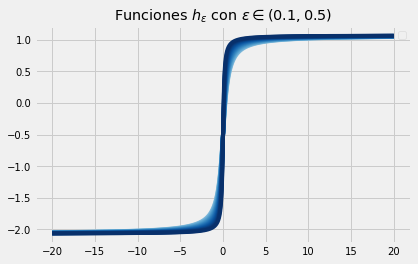
\includegraphics[scale=0.7]{images/p2_h.png}
    \end{figure}
    Obtenemos $\delta'(t)$ 
    \begin{align*}
        \delta'_\epsilon(t) 
        &= \lim_{\epsilon \to 0^+} \delta'_\epsilon(t) \\
        &= \lim_{\epsilon \to 0^+} -\dfrac{2{\epsilon}t}{{\pi}\left(t^2+{\epsilon}^2\right)^2}
    \end{align*}
    \begin{figure}[H]
        \centering
        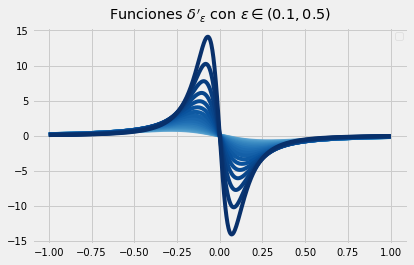
\includegraphics[scale=0.7]{images/p2_f_dot.png}
    \end{figure}
    La gráfica es consistente con la relación:
    \begin{align*}
        \lim_{\epsilon \to 0^+} \int_{-\infty}^\infty \delta'_n g dt &= -g'(0)
        \quad \forall g \in S(R)
    \end{align*}
    Obtenemos $\delta''(t)$:
    \begin{align*}
        \delta''(t) 
        &= \lim_{\epsilon \to 0^+} \delta''_\epsilon(t) \\
        &= \lim_{\epsilon \to 0^+} \dfrac{2{\epsilon}\left(3t^2-{\epsilon}^2\right)}{{\pi}\left(t^2+{\epsilon}^2\right)^3} 
    \end{align*}
    \begin{figure}[H]
        \centering
        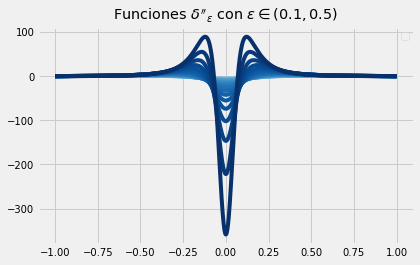
\includegraphics[scale=0.7]{images/p2_f_ddot.png}
    \end{figure}
    La gráfica es consistente con la relación:
    \begin{align*}
        \lim_{\epsilon \to 0^+} \int_{-\infty}^\infty \delta''_n g dt &= g''(0)
        \quad \forall g \in S(R)
    \end{align*}
\end{tcolorbox}
\newpage

\section*{3.-} 
En los siguientes cuatro 4 apartados, a partir de las soluciones
de la ecuación homogénea dadas, obtener una solución particular 
de la ecuación no homogénea usando funciones de Green.
\begin{enumerate}[a)]
    \item $y''-y=sech(x)$, con $sinh(x), cosh(x)$ soluciones de la homogénea.
    \item $x^2y''-2xy'+2y=xlog(x)$, con $x, x^2$ soluciones de la homogénea.
    \item $y''-2cosec^2(x)y=sin^2(x)$, con $cotg(x), 1-xcotg(x)$ soluciones de la homogénea.
    \item $(x^2+1)y''-2xy'+2y=(x^2+1)^2$, con $x, 1-x^2$ soluciones de la homogénea.
\end{enumerate}
\begin{tcolorbox}[breakable]
    \subsubsection*{Caso General}
    En el caso general tenemos la ecuación:
    \begin{align*}
        y''(x) + p(x)y'(x) + q(x)y(x) &= f(x), \quad y(a) = y(b) = 0
    \end{align*}
    la solucuión esta dada por:
    \begin{align*}
        y(x) &= \int_{a}^b G(x,x')f(x')dx'
    \end{align*}
    donde $G$ esta definida por:
    \begin{align*}
        G(x,x') &=
        \begin{cases*}
            A(x')y_1(x), & si $0<x<x'<b$ \\
            B(x')y_2(x),& si $a<x'<x<b$
        \end{cases*}  
    \end{align*}
    donde:
    \begin{align*}
        A &= \frac{y_2}{w} 
        \quad B = \frac{y_1}{w} \\ 
        w &= y_1y_2'-y_1'y_2
    \end{align*}
    con $y_1,y_2$ soluciones de la ecuación homogénea 
    que satisfacen $y_1(a) = y_2(b) = 0$. \\ \\
    Observamos entonces que la solción esta expresada por:
    \begin{align*}
        y &= y_2\int_{a}^x Bf dx' + y_1\int_{x}^b Afdx' 
    \end{align*}
    es importante notar que si $y_1, y_2$ son soluciones de la ecación homogénea
    entonces 
    \[ y = y_1 \pm y_2 \] 
    es solución de la ecuación homogénea.
    \newpage

    \subsubsection*{a)}
    Hacemos cuentas para obtener los parametros del caso general:
    \begin{align*}
        f&= sech \\
        a&=0 &&b=15 \\
        p&=0 &&q=-1 \\
        y_1 &= sinh  &&y_2= cosh(x-b)-1 \\
        y_1' &= cosh &&y_2'=sinh(x-b)
    \end{align*}
    entonces nuestra solución es:
    \begin{align*}
        y &=  y_2\int_{a}^x Bf dx' + y_1\int_{x}^b Afdx' 
    \end{align*}
    resolviendo la integral númericamente obtenemos la gráfica de $y$:
    \begin{figure}[H]
        \centering
        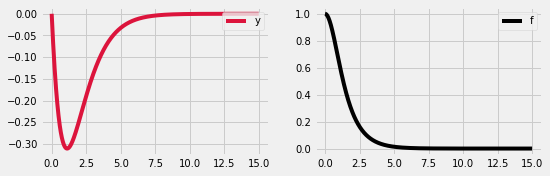
\includegraphics[scale=0.7]{images/p3_1.png}
    \end{figure}

    \subsubsection*{b)}
    Hacemos cuentas para obtener los parametros del caso general:
    \begin{align*}
        f&= \frac{logx}{x} \\
        a&=0 &&b=1 \\
        p&=\frac{-2}{x} &&q= \frac{2}{x^2} \\
        y_1 &= x^2  &&y_2= x^2-x \\
        y_1' &= 2x &&y_2'= 2x-1 
    \end{align*}
    entonces nuestra solución es:
    \begin{align*}
        y &=  y_2\int_{a}^x Bf dx' + y_1\int_{x}^b Afdx' 
    \end{align*}
    resolviendo la integral númericamente obtenemos la gráfica de $y$:
    \begin{figure}[H]
        \centering
        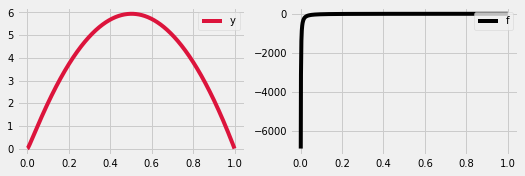
\includegraphics[scale=0.7]{images/p3_2.png}
    \end{figure}

    \subsubsection*{c)}
    Hacemos cuentas para obtener los parametros del caso general:
    \begin{align*}
        f&= sin^2x \\
        a&=0 &&b=\frac{1}{2}\pi \\
        p&=0 &&q= -2cscx^2 \\
        y_1 &= 1-xcotx  &&y_2= cotx \\
        y_1' &= -cotx + xcsc^2x  &&y_2'= -csc^2x 
    \end{align*}
    entonces nuestra solución es:
    \begin{align*}
        y &=  y_2\int_{a}^x Bf dx' + y_1\int_{x}^b Afdx' 
    \end{align*}
    resolviendo la integral númericamente obtenemos la gráfica de $y$:
    \begin{figure}[H]
        \centering
        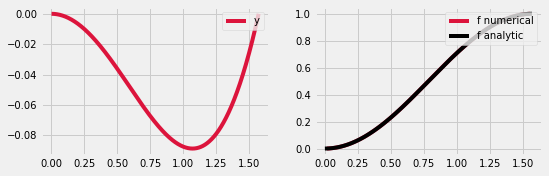
\includegraphics[scale=0.7]{images/p3_3.png}
    \end{figure}

    \subsubsection*{d)}
    Hacemos cuentas para obtener los parametros del caso general:
    \begin{align*}
        f&= x^2+1 \\
        a &=0 &&b=1 \\
        p &=\frac{-2x}{x^2+1} &&q= \frac{2}{x^2+1} \\
        y_1 &=x  &&y_2= 1-x^2 \\
        y_1' &=1 &&y_2'= -2x  
    \end{align*}
    entonces nuestra solución es:
    \begin{align*}
        y &=  y_2\int_{a}^x Bf dx' + y_1\int_{x}^b Afdx' 
    \end{align*}
    resolviendo la integral númericamente obtenemos la gráfica de $y$:
    \begin{figure}[H]
        \centering
        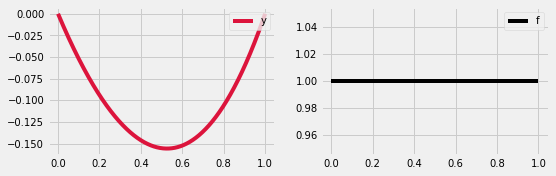
\includegraphics[scale=0.7]{images/p3_4.png}
    \end{figure}
\end{tcolorbox}
\newpage


\section*{4.-}
Resolver las siguientes ecuaciones en derivadas parciales con 
condiciones iniciales usando el método de separación de variables:
\begin{enumerate}[a)]
    \item $\frac{\partial^2u}{\partial x^2}+\frac{\partial^2u}{\partial y^2}+\frac{\partial^2u}{\partial z^2}=0$ en $\Omega=\{(x,y,z)\in \mathbb{R}^3: 0<x,y<c, 0<z<L\}$ con $u(x,y,z)$ anulándose en todos los lados del parlelepípedo excepto en $z=L$ donde $u(x,y,L)=V$.
    \item $-\left(\frac{\partial^2u}{\partial x^2}+\frac{\partial^2u}{\partial y^2}+\frac{\partial^2u}{\partial z^2}\right)=Eu$ en $\Omega=\{(x,y,z)\in\mathbb{R}^3: 0<x<a,0<y<b, 0<z<c\}$
    con $u(x,y,z)$ anulándose en todos los lados del paralelepípedo. 
\end{enumerate}
\begin{tcolorbox}[breakable]
    \subsubsection*{a)}
    Suponemos nuestra solución es de la forma:
    \begin{align*}
        U(x,y,z) &= X(x)Y(y)Z(z)
    \end{align*}
    se tiene entonces:
    \begin{align*}
        \nabla U = U \left( \frac{X''}{X} + \frac{Y''}{Y} + \frac{Z''}{Z}  \right)
    \end{align*}
    por las condiciones del problema se debe de satisfacer:
    \begin{align*}
        \frac{X''}{X} + \frac{Y''}{Y} + \frac{Z''}{Z} &= 0
    \end{align*}
    proponemos las relaciones: 
    \begin{align*}
        -k_n^2 - k_m^2 + k_{nm}^2 &= 0
    \end{align*}
    las solciones a esto son:
    \begin{align*}
        X_n &= 
        \begin{cases}
            sin(k_nx) \\
            cos(k_nx) 
        \end{cases} \\
        Y_m &=
        \begin{cases}
            sin(k_my) \\ 
            cos(k_my)
        \end{cases} \\
        Z_{nm} &=
        \begin{cases}
            sinh(k_{nm}z) \\
            cosh(k_{nm}z)
        \end{cases} 
    \end{align*}
    de acuerdo a las condiciones del problema:
    \begin{align*}
        &U(x,0,z) = 0 &&U(0,y,z) = 0 \\
        &U(x,c,z) = 0 &&U(c,y,z) = 0 \\ 
        &U(x,y,0) = 0 &&U(x,y,L) = V
    \end{align*}
    por lo cual elegimos:
    \begin{align*}
        X_n(x) &= sin\left( \frac{\pi n}{c} x\right) \\
        Y_m(y) &= sin\left( \frac{\pi m}{c} y\right) \\
        Z_{nm}(z) &= sinh(k_{nm}z)
        \quad k_{nm} = \frac{\pi \sqrt{ n^2 + m^2 }}{c} 
    \end{align*}
    ahora bien, proponemos como solución una combinación lineal de nuestras soluciones, esto es:
    \begin{align*}
        U 
        &=\sum_{n=1}^\infty \sum_{m=1}^\infty A_{nm}X_nY_mZ_{nm}
    \end{align*}
    definimos $C_{nm} = A_{nm}Z_{nm}(L)$ y obtenemos la relación:
    \begin{align*}
        U(x,y,L) 
        &=\sum_{n=1}^\infty \sum_{m=1}^\infty C_{nm}X_n(x)Y_m(y)
    \end{align*}
    como $\{\frac{4}{c^2}sin(\frac{\pi n}{c}x)sin(\frac{\pi m}{c}y),\quad n,m \in N\}$ son base ortonormal del espacio 
    de funciones continuas de périodo $c$ en $x$ y $y$:
    \begin{align*}
        C_{nm} &= \frac{4}{c^2} \int_0^c\int_0^c Vsin\left(\frac{\pi n}{c}x\right)sin\left(\frac{\pi m}{c}y\right)dxdy
    \end{align*}
    haciendo cuentas encontramos:
    \begin{align*}
        A_{nm} &= 
        \begin{cases}
        \frac{16V}{nm\pi^2}\frac{1}{sinh(k_{nm}L)} & m,n \in impares \\
        0 &c.c    
        \end{cases}
    \end{align*}
    \subsubsection*{b)}
    Nuevamente calculando el gradiente obtenemos:
    \begin{align*}
        \frac{X''}{X} + \frac{Y''}{Y} + \frac{Z''}{Z} &= -E
    \end{align*}
    proponemos las relaciones:
    \begin{align*}
        -k_n^2 -k_m^2 -k_{l}^2 &= -E
    \end{align*} 
    dada las condiciones del problema elegimos:
    \begin{align*}
        X_n(x) &= sin\left( \frac{\pi n}{a} x\right) \\
        Y_m(y) &= sin\left( \frac{\pi m}{b} y\right) \\
        Z_{l}(z) &= sin\left( \frac{\pi l}{c} z\right)
    \end{align*}
    entonces tenemos un conjunto de soluciones:
    \begin{align*}
        U_{nml} &= X_nY_mZ_l 
    \end{align*}
    que satisfacen:
    \begin{align*}
        -\nabla^2 U_{nml} &= E_{nml} \\ 
        E_{nml} &= k_n^2+k_m^2+k_l^2 
    \end{align*}
    tambien cualqueir multiplicación por un escalar de estas solcuiones sigue siendo 
    solución al problema, en el caso de que $E$ no se pueda ver de esta forma se tiene
    la solución trivial $U=0$.
\end{tcolorbox}
\section*{Bibliografía}
\begin{itemize}
    \item \textit{Mathematical Methods in the Physical Sciences}. Boas, Mary. Tercera Edición. Lehigh Press. 2006. Cap.
\end{itemize}

\end{document}